\documentclass{article}
\usepackage[margin=1in]{geometry}
\title{Minutes from 17 August}

\usepackage{float}
\usepackage{amsmath}
\usepackage{tikz}
\usetikzlibrary{positioning, arrows}

\begin{document}
\section{Papers referred to}
\begin{enumerate}
	\item Marie-Sarah Lacharite, Brice Minaud. \textbf{Improved Reconstruction Attacks on Encrypted Data Using Range Query Leakage}

	\item \textbf{K-Nearest-Neighbour Search on Encrypted Data} (Not published yet)
	
	\item Rafail Ostrovsky. \textbf{Software Protection and Simulation on Oblivious RAMs}
	
	\item Data structure and algorithms I have learnt during undergraduate.
\end{enumerate}


\section{A new OPE scheme}
\begin{itemize}
	\item The idea is to use `searchable' data structures to pre-process the queries so that the queries do not leak the sets used in 1.
	
	\item Sketch of the scheme:
	\begin{figure}[H]
		\begin{center}
			\includegraphics[width=1.0\textwidth]{./new_scheme.jpg}
		\end{center}
	\end{figure}

	\item Instead of lookup table to identify the block to retrieve, one can use PRF on the endpoints (in terms of range covered by the block) of the block.
	
	\item Claim: the block returned contains at most twice number of items than the actual items.
	
	\item Problems with the scheme:
	\begin{itemize}
		\item The claim is not quite true: consider the range spanning the second and third block in the bottom layer, there is no single block to return from the layer on top. However, there is a simple fix to this, and does not change space complexity (\textbf{To be discussed in the next meeting}).
		
		\item If the range is 1 to $2^k$ then this scheme is not ideal in terms of space complexity. I claim that the scheme can be modified to achieve a very low overhead (\textbf{To be discussed in the next meeting}).
	\end{itemize}
	
	\item To think: what does the scheme leak?
\end{itemize}


\section{ORAM}
\begin{itemize}
	\item Confirms that the lower-bound of overhead is indeed $\mathcal{O}(\log{n})$.
	
	\item Question to be answered: is ORAM any similar to OPE in the sense that, in order to hide access pattern, how much overhead does it cost?
\end{itemize}


\section{Syntax of encrypted database}
\begin{itemize}
	\item We can think of database in three levels: a string of zeros and ones in the most abstract form, a database as a set of strings, and a database with all the details.
	
	\item We will formalize syntax on the most abstract form first.
	
	\item Notation (need better names):
	\begin{itemize}
		\item \textbf{Initialise}: $1^\lambda \rightarrow \text{params}^{*}$
		
		\item \textbf{KeyGen}: $1^\lambda \rightarrow \textbf{sk}$
		
		\item \textbf{Enc}: $1^\lambda \times \textbf{sk} \times \textbf{DB} \rightarrow \textbf{EDB}$
		
		\item \textbf{Dec}: $1^\lambda \times \textbf{sk} \times \textbf{EDB} \rightarrow \textbf{DB}$
		
		
		\item $\mathcal{Q}$: $\textbf{DB} \times Q \rightarrow \textbf{DB}$
		
		\item \textbf{encQ}: $1^\lambda \times \textbf{sk} \times Q \rightarrow \textbf{eQ} \times \textbf{iQ}$
		
		\item \textbf{EQ}: $1^\lambda \times \textbf{sk} \times \textbf{EDB} \times \textbf{eQ} \rightarrow \textbf{EDB}$
		
		\item \textbf{DQ}: $1^\lambda \times \textbf{sk} \times \textbf{EDB} \times \textbf{iQ} \rightarrow \textbf{DB}$
	\end{itemize}

	\item Additional notation:
	\begin{itemize}
		\item $\Pi_i$: projection of $i$-th component of the arguments
		\item $id$: identity function
	\end{itemize}

	\item Commutative diagram:
	\begin{figure}[H]
		\begin{center}
			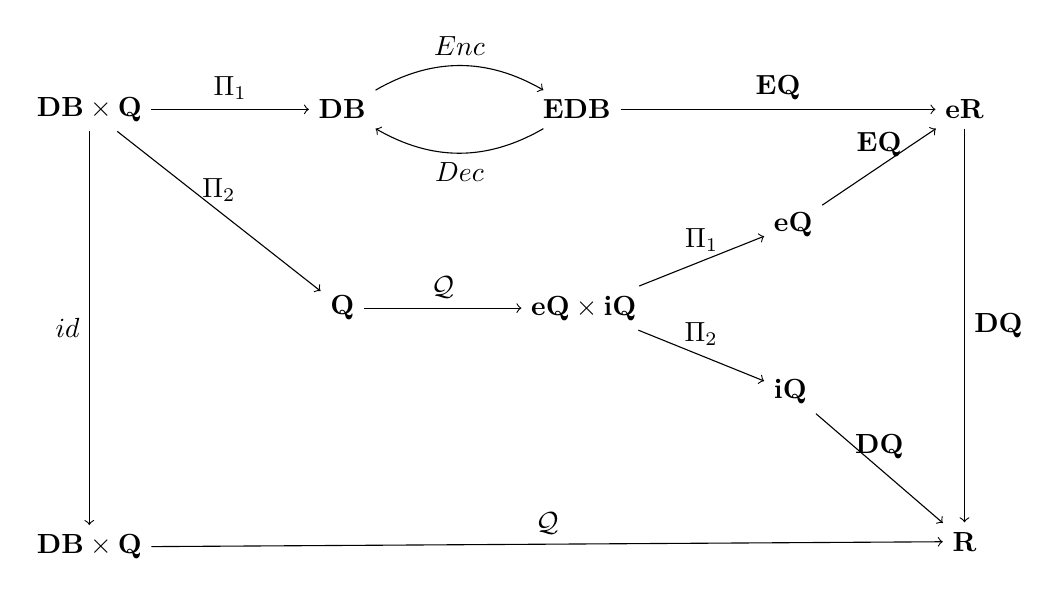
\begin{tikzpicture}[->,node distance = 2cm, auto]
				\node (init)                                         {$\textbf{DB} \times \textbf{Q}$};
				\node (DB)   [right = of init]                       {$\textbf{DB}$};
				\node (EDB)  [right = of DB]                         {$\textbf{EDB}$};
				
				\node (Q)    [below = of DB]                         {$\textbf{Q}$};
				\node (eiQ)  [right = of Q]                          {$\textbf{eQ} \times \textbf{iQ}$};
				\node (eQ)   [above right = 0.5cm and 1.5cm of eiQ]  {$\textbf{eQ}$};
				\node (iQ)   [below right = 0.5cm and 1.5cm of eiQ]  {$\textbf{iQ}$};
				
				\node (eR)   [right = 4cm of EDB]                    {$\textbf{eR}$};
				\node (R)    [below = 5cm of eR]                     {$\textbf{R}$};
				
				\node (void) [below = 5cm of init]                   {$\textbf{DB} \times \textbf{Q}$};
				
				\path
				(init) edge node[above] {$\Pi_1$}           (DB)
				(DB)   edge[bend left] node[above] {$Enc$}  (EDB)
				(EDB)  edge[bend left] node[below] {$Dec$}  (DB)
				(EDB)  edge node[above] {$\textbf{EQ}$}     (eR)
				(eR)   edge node[right] {$\textbf{DQ}$}     (R)
				
				(init) edge node[above] {$\Pi_2$}           (Q)
				(Q)    edge node[above] {$\mathcal{Q}$}     (eiQ)
				(eiQ)  edge node[above] {$\Pi_1$}           (eQ)
				(eiQ)  edge node[above] {$\Pi_2$}           (iQ)
				(eQ)   edge node[above] {$\textbf{EQ}$}     (eR)
				(iQ)   edge node[above] {$\textbf{DQ}$}     (R)
				
				(init) edge node[left] {$id$} (void)
				(void) edge node[above] {$\mathcal{Q}$}     (R)
				;
				
			\end{tikzpicture}
		\end{center}
	\end{figure}
	
	
\end{itemize}




\end{document}